\chapter{Methodology}
\label{sec:methodology}
% Focus on what you add to the existing method. Explain what you will do and why (and how). Do not forget to characterize your research design. There should be a sub-section on the evaluation. 
%For DS students, this normally means using manually labelled or ground truth data. For IS students, it is not always needed to have a separate methodology section. You can also integrate the approach with the results in one section. It depends on your type of research what is best fitting.
%Write about your methodology here. Focus on your own contribution. Indicate exactly how you will assess your work in terms of evaluation.

% It is possible to use a separate section for the Experimental Setup, which then focuses on all settings used in your experiments. It also possible to address the settings in a sub-section under Methodology. 
%\section{Equations}
%        We estimate the deformable template parameters~$\theta_t$ and the deformation fields for every data point using maximum likelihood. Letting~$\mathcal{V} = \{\boldsymbol{v}_i\}$ and~$\mathcal{A} = \{a_i\}$,
        %
%        \begin{align}
%                \hat{\theta_t}, \hat{\mathcal{V}} &= \arg \max_{\theta_t, \mathcal{V}} \log p_{\theta_t}(\mathcal{V} | \mathcal{X},  \mathcal{A}) \nonumber \\
%                &= \arg \max_{\theta_t, \mathcal{V}} \log p_{\theta_t}(\mathcal{X} | \mathcal{V}; \mathcal{A}) + \log p(\mathcal{V}),
%                \label{eq:logpost}
%        \end{align}
        %
%        where the first term captures the likelihood of the data and deformations, and the second term controls a prior over the deformation fields.

%        \begin{proof}
%                Awesome proof.
%        \end{proof} 

%\section{Long equations in two columns}
%        Note that equations can fill the width pretty quickly when there are two columns.
%        Different mathemtical environments, beyond the basic \verb|\begin{equation}| may be of use. Taking as an example the binomial formula which overflows in Eq. \eqref{binom:eq}:
%        \begin{equation}
%                \label{binom:eq}
%                (1+x)^n = \underbrace{(1+x)\times...\times(1+x)}_{n \text{ times}} = \sum_{k=0}^n \binom{n}{k}x^k = \sum_{k=0}^n\frac{n!}{k!(n-k)!}x^k .
%        \end{equation}

%        The \verb|\begin{multline}| environment is an easy although crude fix:
%        \begin{multline}
 %               (1+x)^n = \underbrace{(1+x)\times...\times(1+x)}_{n \text{ times}} \\
 %               = \sum_{k=0}^n \binom{n}{k}x^k \\
 %               = \sum_{k=0}^n\frac{n!}{k!(n-k)!}x^k .
 %       \end{multline}
 %       \verb|\begin{align}| tends to give the most control over the final result:
 %       \begin{align}
%                (1+x)^n &= \underbrace{(1+x)\times...\times(1+x)}_{n \text{ times}} \nonumber\\
%                        &= \sum_{k=0}^n \binom{n}{k}x^k \nonumber\\
%                        &= \sum_{k=0}^n\frac{n!}{k!(n-k)!}x^k .
%        \end{align}


%\section{Math styles}
%        Different font styles can be used for equations:
%        \begin{itemize}
%                \item \verb|$a b c A B C 1 2 3$|: $ a b c A B C 1 2 3 $
%                \item \verb|$\mathbf{a b c A B C 1 2 3}$|: $ \mathbf{a b c A B C 1 2 3} $
%                \item \verb|$\mathfrak{a b c A B C 1 2 3}$|: $ \mathfrak{a b c A B C 1 2 3} $
%                \item \verb|$\mathcal{ABC}$|: $ \mathcal{ABC} $
%                \item \verb|$\mathbb{ABC}$|: $ \mathbb{ABC} $
%                \item \verb|$\mathsf{ABC}$|: $ \mathsf{ABC} $
%                \item \verb|$\mathtt{ABC}$|: $ \mathtt{ABC} $
%        \end{itemize}

%        Text and names in equations should be dealt with the \verb|\text| command, for instance:\\
%        \verb|$\mathcal L_{\text{SuperLoss}}$|: $\mathcal L_{\text{SuperLoss}}$ and not $\mathcal L_{SuperLoss}$.


\section{Overview}

Our benchmark evaluates tool synthesis end-to-end: a synthesis agent reads API documentation and produces an MCP server; a separate evaluation agent attempts natural-language tasks against that server; an LLM judge scores each attempt. The three-stage design cleanly separates synthesis quality from agent reasoning ability, allowing failures to be attributed to the correct component. The process is fully automated and requires no human annotation beyond the initial task authoring. Figure~\ref{fig:pipeline} illustrates the pipeline.

\begin{figure}[h]
\centering
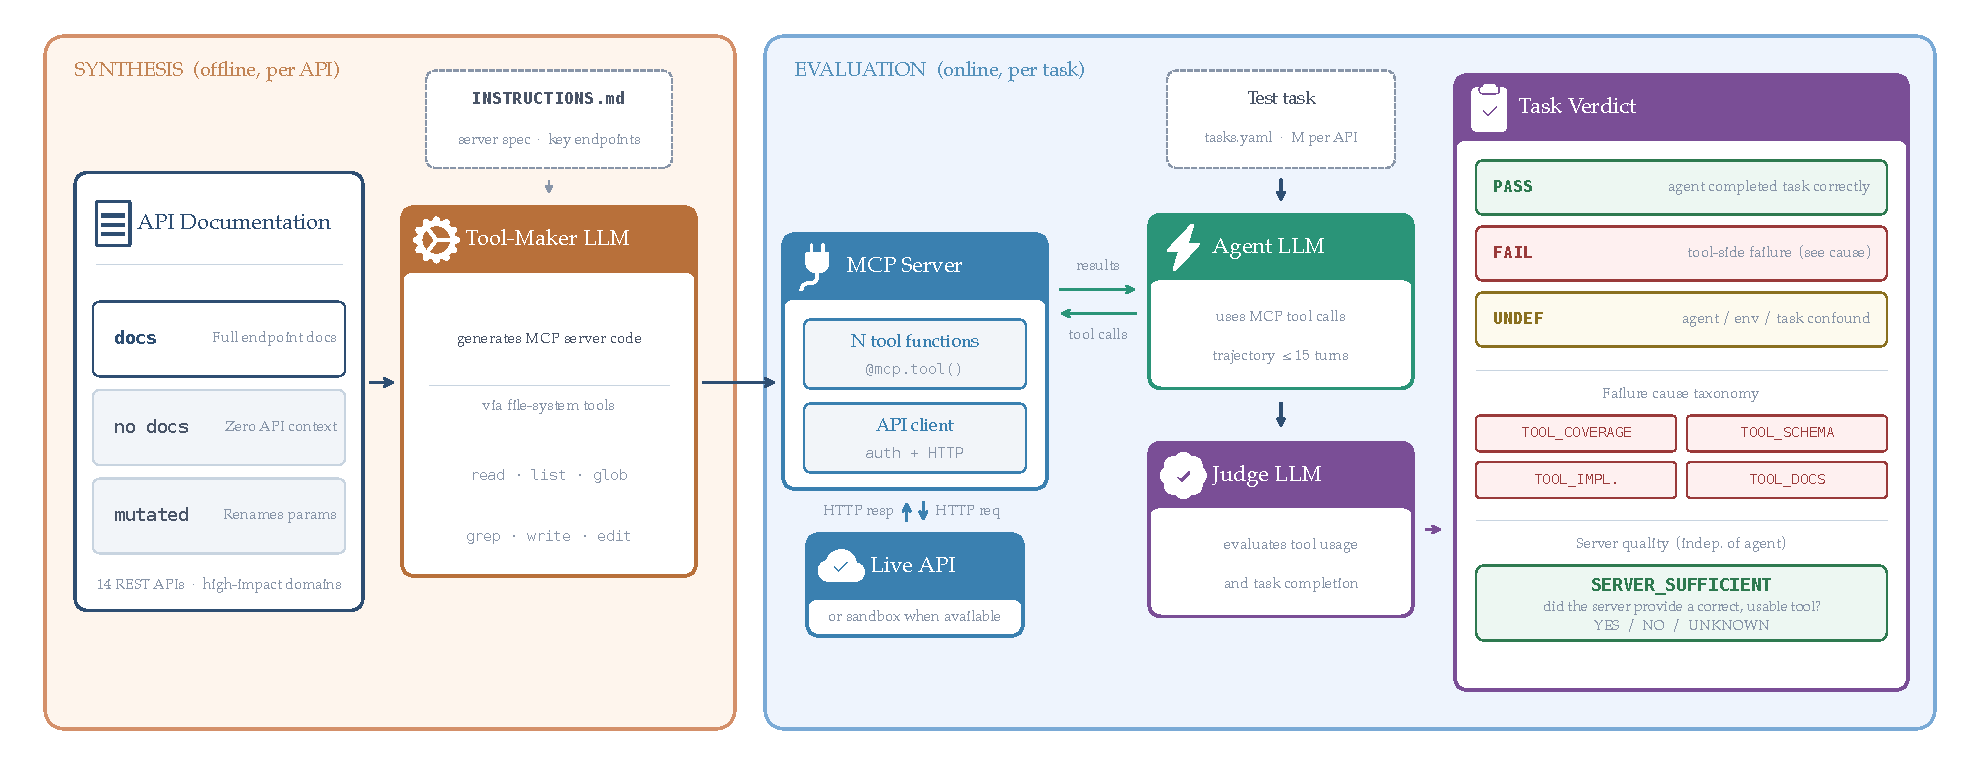
\includegraphics[width=\linewidth]{media/benchmark_pipeline_thesis_v4.pdf}
\caption{End-to-end benchmark pipeline. A synthesis agent reads documentation and produces an MCP server; a separate evaluation agent attempts tasks against it; a judge scores each attempt.}
\label{fig:pipeline}
\end{figure}

\noindent
This separation is the central design choice. In prior tool-use evaluations, the tool layer is given; here it is produced under test. A synthesized server that crashes, exposes incomplete tool coverage, or maps arguments incorrectly will cause agent failures regardless of how capable the evaluation model is. By isolating the synthesis stage, we can attribute failures to either the tool infrastructure (synthesis failures) or the evaluation agent (reasoning failures), and measure how tightly the two are coupled.

\section{Benchmark Datasets}

\subsection{API Selection}

We select 14 REST APIs spanning five domains: developer tooling (GitHub), productivity and collaboration (Notion, Confluence, Jira), e-commerce (eBay Buy, eBay Commerce, eBay Sell, Shopify), communication (Mastodon, Zulip), and data and financial services (Stripe, Alphavantage, Spoonacular, OpenWeatherMap). Selection criteria were: (i)~availability of a sandboxed or resettable test environment with stable test credentials, (ii)~REST-based HTTP interface returning JSON, (iii)~public developer documentation available as HTML or Markdown, and (iv)~variation along the two primary experimental axes: \emph{familiarity} (the degree to which an API is likely well-represented in pre-training corpora) and \emph{complexity} (endpoint count, parameter density, and authentication complexity).

APIs range from high-familiarity, high-complexity (GitHub, Stripe) to low-familiarity, low-complexity (Alphavantage, OpenWeatherMap). The eBay suite provides three difficulty tiers within a single platform: the Buy, Commerce, and Sell sub-APIs differ substantially in documentation volume and endpoint coverage despite sharing the same host and OAuth model. Jira and the eBay Sell API represent the most challenging synthesis targets, with large hierarchical documentation and high parameter cardinality.

\subsection{Documentation Collection}

For each API, we scrape the official developer documentation portal and convert it to Markdown using a DOM-to-Markdown pipeline. Depending on the API's documentation structure, this produces between 7 and 190 Markdown files per dataset (median approximately 35 files). Files range from single-endpoint reference pages to category-level overview pages covering multiple related endpoints. We do not post-process or selectively filter the scraped content beyond format normalisation; the synthesizer receives the documentation in the same form it appears online, including navigation artefacts, code samples in multiple languages, and pagination boilerplate.

This choice is deliberate: it reflects realistic synthesis conditions, where a practitioner points a synthesis agent at a raw documentation URL rather than a curated, cleaned API description. The resulting noise is part of the synthesis challenge the model must handle.

\subsection{Human Reference Servers}

For two APIs --- GitHub and Zulip --- publicly available, community-maintained MCP servers exist and can be evaluated against the same task suite. The GitHub MCP server is the official implementation maintained by GitHub; the Zulip server is a community-contributed open-source project. Both are written in TypeScript using the official MCP SDK and expose a subset of the respective APIs as tools. We run both reference servers against the same evaluation agent and judge pipeline used for the synthesized servers, without any modification.

These human-authored servers serve as a practical baseline: they represent what a developer with API familiarity and access to the official documentation would produce without time pressure from an automated benchmark. Crucially, neither server was constructed with our specific evaluation tasks in mind, so coverage gaps reflect genuine tool-design choices rather than benchmark overfitting. Comparing synthesized server PASS rates against these baselines directly answers whether automated synthesis can match or exceed hand-crafted implementations (Section~\ref{sec:rq2}).

\subsection{Parameter Mutations}

To probe the degree to which synthesis models rely on parametric knowledge rather than the provided documentation, we introduce a \emph{mutated} condition ($C_{\text{mut}}$) for each API. For each dataset, we identify 4--6 core parameter names that are prominent in the API and likely encoded in training-time weights (e.g.\ \texttt{limit}, \texttt{offset}, \texttt{sort} for eBay Buy) and replace them uniformly throughout the documentation with plausible but distinct alternatives (e.g.\ \texttt{max\_results}, \texttt{skip}, \texttt{order\_by}). Replacement names are chosen to be syntactically plausible --- consistent with conventions in adjacent APIs --- while being clearly different from the originals at the string level.

A synthesis model that faithfully follows the mutated documentation should produce tools using the new parameter names consistently. A model dominated by parametric memory will reproduce the original names regardless. We quantify this as \emph{mutation adherence}, measured at two levels:

\begin{itemize}
  \item \textbf{Interface adherence}: the mutated name appears as a Python
    identifier in the MCP tool function signature, i.e.\ the evaluation agent
    sees and receives the renamed parameter.
  \item \textbf{HTTP adherence}: the mutated name appears as a quoted string
    key in the outbound HTTP request. This is a stricter criterion; a model
    may adopt the renamed identifier locally but revert to the original name
    when constructing the HTTP payload.
\end{itemize}

\noindent
HTTP adherence is always $\leq$ interface adherence. The gap between the two is informative: a large gap indicates the model partially follows documentation (adopting Python argument names) but reverts to training priors when constructing HTTP calls.

To enable fair PASS comparison across conditions, we apply a \emph{patch} step to mutated servers before evaluation: the original parameter names are restored in the source files, so the evaluation agent always calls the real API with the correct parameters regardless of whether the synthesizer adopted the mutations. Adherence is measured before patching; PASS is measured after.

\section{Synthesis Pipeline}

\subsection{Task Specification}

Each dataset includes a \texttt{TASK.md} file that provides the synthesis agent with all information needed to produce a functional server. The
specification covers: the target implementation framework (FastMCP for Python,
or the official \texttt{@modelcontextprotocol/sdk} for TypeScript), the list of available documentation files and their location, required environment variables (API keys, OAuth credentials, sandbox flags), authentication flow (typically OAuth~2.0 client credentials or a static API key), coverage expectations (broad CRUD on core resource types, support for multi-step workflows), and required deliverables.

Deliverables are uniform across all datasets and language choices:
\begin{itemize}
  \item \texttt{server.py} (or \texttt{server.ts}): the MCP entry point that
    registers all tools and starts the stdio server.
  \item \texttt{requirements.txt} (or \texttt{package.json}): pinned
    dependencies for reproducible installation.
  \item \texttt{grounding.json}: a manifest mapping every synthesized tool
    name to the source documentation file and HTTP endpoint it implements
    (e.g.\ \path{\{"doc": "docs/browse.md", "endpoint": "GET /buy/browse/v1/item\_summary/search"\}}).
\end{itemize}

\noindent
The grounding manifest enables two lightweight analyses. \emph{Citation validity} checks that each entry's \texttt{doc} field names a file that exists in the documentation corpus and that the \texttt{endpoint} field contains a syntactically plausible HTTP method--path string. \emph{Grounding coverage} checks that every synthesized tool has a corresponding entry --- i.e.\ the synthesizer claimed a source for each tool it produced. These checks do not verify that the implementation is faithful to the cited documentation, only that the synthesizer anchored each tool to \emph{some} real document and endpoint rather than producing an entry-free, free-form stub.

\subsection{Synthesis Agent}

The synthesis agent operates in an agentic loop with access to a set of file-system tools. The primary synthesis models (GPT-5.2, GPT-5.4, and Qwen3-Coder-Next via vLLM) are provided six tools: \texttt{read\_file}, \texttt{write\_file}, \texttt{edit\_file}, \texttt{glob}, \texttt{grep}, and \texttt{list\_directory}. The agent receives the task specification and, depending on the synthesis condition, a populated documentation directory. It iterates freely until it produces the required deliverables.

A typical synthesis run follows three phases. In the \emph{exploration} phase (turns 1--3), the agent reads \texttt{TASK.md}, lists the documentation directory, and reads a subset of files to understand the API's structure and authentication model. In the \emph{implementation} phase (turns 4--20), it writes tool modules and a shared HTTP client. In the \emph{finalisation} phase (last 2--3 turns), it assembles \texttt{server.py}, writes
\texttt{grounding.json} and \texttt{requirements.txt}, then performs a self-verification pass by rereading key files. Figure~\ref{fig:synth-trace} shows a representative trace.

\begin{figure}[h]
\centering
\small
\begin{verbatim}
[turn 1]  read_file(TASK.md)
[turn 1]  glob(docs/*.md)
[turn 2]  read_file(docs/browse.md)
[turn 2]  read_file(docs/item.md)
[turn 4]  write_file(generated_tools/browse.py)
[turn 7]  write_file(generated_tools/order.py)
[turn 9]  write_file(server.py)
[turn 10] write_file(grounding.json)
[turn 11] write_file(requirements.txt)
\end{verbatim}
\caption{Typical synthesis agent trace (eBay Buy, docs condition, GPT-5.2). 813K input tokens, 11K output tokens, 190 seconds.}
\label{fig:synth-trace}
\end{figure}

\noindent
GPT-class synthesizers tend to produce a two-layer architecture: a \texttt{generated\_tools/} directory of domain-specific Python modules (e.g.\ \texttt{issues.py}, \texttt{pulls.py} for GitHub), each implementing a group of related endpoints through a shared HTTP client, with \texttt{server.py} acting as a thin registration layer applying \texttt{@mcp.tool()} decorators. Qwen3-Coder-Next typically produces a flat structure with all tool logic in a single \texttt{server.py}. Both patterns are accepted by the evaluation harness; only the MCP interface contract matters for evaluation.

\subsection{Synthesis Conditions}

We evaluate each API under three synthesis conditions, corresponding to three
instantiations of the context $C$ in Equation~\ref{eq:synthesis}:

\begin{itemize}
  \item $C_{\text{docs}}$ \textbf{(with docs)}: the agent receives all
    scraped documentation files in addition to the task specification.
  \item $C_{\emptyset}$ \textbf{(no docs)}: the agent receives only the
    task specification, with no documentation. All tool implementations must
    come from parametric knowledge.
  \item $C_{\text{mut}}$ \textbf{(mutated docs)}: the agent receives the
    mutated documentation, creating a controlled conflict between in-context
    parameter names and training-time priors.
\end{itemize}

\noindent
Synthesis resource usage varies substantially across conditions. GPT-5.2 docs-condition runs typically require 15--25 agent turns, consuming 14K--2.4M input tokens (reflecting documentation corpus size, which ranges from 7 to 190 files). No-docs runs are substantially shorter: 14K--24K input tokens and approximately 1 minute wall time, since the agent skips document reads and writes directly from parametric memory.

\subsection{Synthesis Models}

We evaluate five synthesis models. GPT-5.2 serves as the primary baseline, run across all 14 APIs and all three conditions. GPT-5.4 is run across all 14 APIs as a more recent baseline. Sonnet~4.6 (Claude Sonnet) is run across a representative subset of APIs. Gemini~3.1~Pro provides a third model family for comparison. Qwen3-Coder-Next is run locally via a vLLM inference server. These span a range of training corpora, post-training regimes, and context window sizes, allowing us to assess whether synthesis quality is model-specific or reflects a more general capability. Model comparison results are presented
in Section~\ref{sec:rq1}.

\section{Evaluation Framework}

\subsection{Evaluation Tasks}

For the 14 APIs in the primary evaluation set, we manually authored 13--25
natural-language tasks per API (265 tasks total; median 19 per API). Tasks
are specified in a \texttt{tasks.yaml} file using a four-field schema:

\begin{verbatim}
- id: search_products
  prompt: >
    Search for "wireless headphones" on eBay. Report
    the title, price, and item ID of the first 5
    results.
  expected: itemId
  tags: [read]
\end{verbatim}

\noindent
Tasks follow four design principles. First, prompts are \emph{goal-oriented}: they describe the desired outcome without naming tools, parameter fields, or HTTP endpoints. Second, they provide only the domain knowledge the agent cannot infer from tool schemas (e.g.\ ``amounts are in cents''), not call sequences or parameter names. Third, they require \emph{synthesis over echo}: comparison, counting, filtering, or multi-step retrieval rather than raw
response reporting. Fourth, chain depth is capped at six sequentially dependent calls, with the intended range being 2--4 steps.

The \texttt{expected} field contains a task-specific substring --- typically a field name, ID, or derived value --- that can only appear in the agent's final answer if it called the correct tool with semantically correct parameters. This string is passed to the judge as a ground-truth hint, reducing ambiguity in open-ended response scoring.

Tasks are distributed across four functional categories: smoke tests (single-call reads verifying basic tool reachability), multi-step workflows (search then retrieve, create then verify), error-handling tasks (invalid IDs, missing resources, permission boundaries), and harder synthesis tasks requiring pagination, cross-resource joins, or derived computations. Write tasks use a consistent naming prefix (e.g.\ \texttt{"Agent Eval Test *"}) to facilitate cleanup and prevent cross-run contamination.

\subsection{Evaluation Agent}

The evaluation agent (Gemini~2.5~Pro) connects to the synthesized MCP server via stdio transport and executes an agentic loop. At each turn it receives the full message history --- system prompt, task prompt, and all prior tool results as \texttt{ToolMessage} objects --- and responds with either a set of tool calls or a final textual answer. The loop terminates when the model emits a response with no tool calls, or after a maximum of 15 turns.

The agent's system prompt instructs it to always call at least one tool before answering, use observed tool results to inform subsequent calls, and pass environment-specific constants (e.g.\ \texttt{EBAY\_ENVIRONMENT=SANDBOX}) verbatim rather than inferring them. The prompt does not describe individual tools or their signatures; the agent discovers available tools at runtime by calling \texttt{list\_tools()}. The agent does not perform explicit chain-of-thought reasoning steps between tool calls; reasoning is implicit in the model's generation.

The evaluation harness speaks only MCP: it calls \texttt{list\_tools()} to discover available tools and \texttt{call\_tool(name, args)} to invoke them.
No other protocol or API client is provided. All HTTP logic --- authentication, request construction, token refresh, error handling --- executes inside the synthesized server process and is invisible to both the harness and the evaluation agent. The evaluation agent's performance therefore depends entirely on the interface quality and implementation correctness of the synthesized server.

\subsection{Judge}

Task outcomes are assessed by a separate LLM judge (Gemini~3~Flash) that does not participate in the agentic loop. The judge receives a structured prompt containing four components: the original task prompt, the list of all tool names and their one-line descriptions (from \texttt{list\_tools()}), the full tool-call trajectory formatted as numbered steps (\texttt{Step N: tool\_name(\{args\}) $\rightarrow$ [truncated result]}), and the agent's final textual answer. It is asked three questions:

\begin{enumerate}
  \item \textbf{OUTCOME}: Did the agent complete the task correctly?
    (\textsc{pass} / \textsc{fail})
  \item \textbf{FAILURE\_CAUSE}: If \textsc{fail}, what was the primary cause?
    One of eight codes:
    \textsc{tool\_coverage} (required tool absent from server),
    \textsc{tool\_documentation} (tool present but name or description
    prevented the agent from identifying it),
    \textsc{tool\_schema} (tool present but parameters incorrectly typed
    or named),
    \textsc{tool\_implementation} (tool called correctly but returned wrong
    or malformed data),
    \textsc{agent\_reasoning} (tools were sufficient but agent misused them),
    \textsc{task\_ambiguous} (task wording unclear or contradictory),
    \textsc{environment} (server crash, network error, credential failure),
    \textsc{none} (used when \textsc{outcome} is \textsc{pass}).
  \item \textbf{SERVER\_SUFFICIENT}: Setting aside what the agent did,
    did the synthesized server provide all tools needed to complete the task?
    (\textsc{yes} / \textsc{no} / \textsc{unknown})
\end{enumerate}

\noindent
The judge responds in a fixed plain-text format (no markdown) to enable reliable parsing:

\begin{verbatim}
OUTCOME: PASS
FAILURE_CAUSE: NONE
SERVER_SUFFICIENT: YES
REASON: The agent correctly identified the search tool, 
        applied the right filters, and extracted the 
        requested itemId values.
\end{verbatim}

\noindent
The \textsc{tool\_documentation} category distinguishes a missing tool (coverage gap) from a present-but-undiscoverable tool (documentation gap): when the server implements the correct endpoint but gives it a misleading name or description, the agent fails not because the tool is absent but because it cannot identify it. This distinction is absent from most prior tool-use benchmarks and matters for understanding where synthesis quality breaks down independent of coverage.

\subsection{Metrics}
\label{sec:metrics}

We report two primary metrics derived from the judge's structured output.

\textbf{PASS} is the fraction of task attempts scored \textsc{pass} out of all \emph{scoreable} attempts. A task attempt is excluded from the denominator if it is attributed to \textsc{environment} (external infrastructure failure unrelated to synthesis quality) or \textsc{task\_ambiguous} (measurement
confound). Failures attributed to \textsc{agent\_reasoning} are also excluded:
they count neither as pass nor fail, because they reflect the evaluation agent's behaviour rather than the synthesized server. PASS is thus a clean signal about tool infrastructure quality:
%
\begin{equation}
  \text{PASS}
  = \frac{\#\,\textsc{pass}}
    {\#\,\textsc{pass} + \#\,\textsc{fail}_{\text{tool}}}
  \label{eq:pass}
\end{equation}
%
where $\#\,\textsc{fail}_{\text{tool}}$ counts failures attributed to
\textsc{tool\_coverage}, \textsc{tool\_documentation},
\textsc{tool\_schema}, or \textsc{tool\_implementation}.

\textbf{SYNTH} (synthesis sufficiency) is derived from the \textsc{server\_sufficient} verdict: it is the fraction of tasks for which the judge found the server sufficient regardless of whether the agent succeeded. SYNTH measures synthesis quality independently of the evaluation
agent, and is computed only for tasks where the judge returned a non-\textsc{unknown} verdict. When SYNTH is high but PASS is low, the bottleneck is agent reasoning; when both are low, the bottleneck is synthesis.

Together, the two metrics place each API--condition data point in one of three regimes: \emph{synthesis-limited} (low SYNTH, low PASS), \emph{agent-limited} (high SYNTH, lower PASS), or \emph{ceiling} (high SYNTH, high PASS). The scatter plot of SYNTH against PASS (Section~\ref{sec:rq5}) visualises this decomposition across all 42 API--condition pairs in the primary evaluation.
